\chapter{Conclusion}
\label{chapter-conclusion} 

\section{Summary of work done}

In the first semester, the main objective is to develop proficiency in the necessary theoretical foundation and implementation skills. These included tensor CP decomposition, diffusion map, and persistent homology. To gain better intuition, I demonstrated each of the methods on toy data sets such as face image data and MNIST \cite{mnist}. 

Due to the interdisciplinary nature of the project, much time is also spent studying the theoretical foundations of computational neuroscience. This includes the history of computational models of the visual system and the connections with mathematical and computational ideas. 

I have also conducted many exploratory experiments. A complete list of the experiments are included below.
For the biological neural tensor, I conducted the following experiments:
\begin{enumerate}
    \item applying tensor CP decomposition to generate the neural manifold
    \item applying diffusion map to generate the neural manifold
    \item applying persistent homology and Wasserstein distance to compare the topological features of the neural manifold
\end{enumerate}

For the artificial neural tensor, I conducted the following experiments:
\begin{enumerate}
    \item building the artificial neural tensor without considering shifts in images
    \item building the artificial neural tensor with shifts in images
    \item applying tensor CP decomposition on the artificial neural tensor (with shifts in images)
    \item studying how the neural manifold changes during the training of an ANN (instead of using the pre-trained ANN)
    \item applying persistent homology (though with limited explainability)
\end{enumerate}

In all, I am on track with the timeline and have completed more than the plans we laid out at the beginning of the semester.  A bird-eye view of the work done during the first semester is shown in the figure below.

\begin{figure}[H]
        \centering
     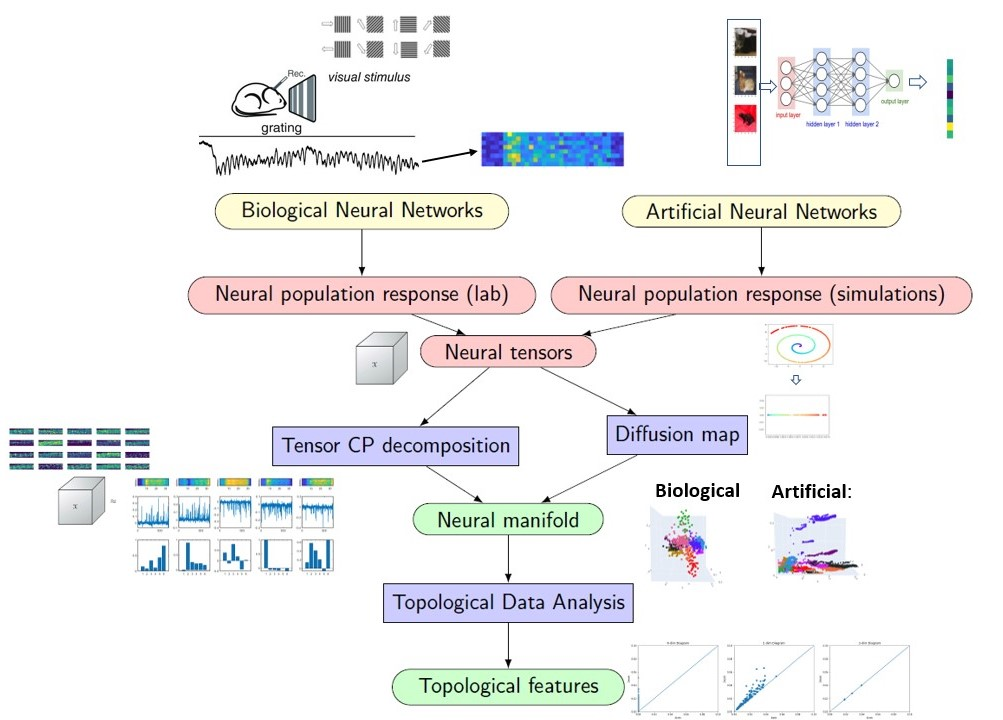
\includegraphics[width=1.2\textwidth]{presentation/Slide4.jpg}
        \end{figure} 
        
\section{Next steps}
In the past few months, I have finished learning the foundations behind the methods and applying these methods to conduct relevant experiments using the neural tensors from the lab neural spiking data and the pre-trained VGG-16 model.  

Given the progress made, I propose the following next steps:
\begin{itemize}
    \item Provide more thorough and rigorous interpretations of the results for CNN. This will likely involve more sophisticated understanding of theoretical neuroscience, which could be addressed by reading the book on neuromathemtics and talking to the co-supervisor who is working directly in this area. 
    \item Apply the same methods to RNN to investigate whether there would be any interesting differences.
    \item Come up with a way to quantify the differences between neural manifolds. This could potentially be done by using persistent homology and the Wasserstein distance.
    \item Implement diffusion map on the artificial neural tensors with the appropriate parameters.
    \item Identify a potential novelty that this project could offer, which would be a contribution that is not in the research literature before. This could be some interesting results from the experiments, or a proposal of a new improvement to the existing methodology. 
\end{itemize}


